In this section,
the proposed \DAIL{} agent is introduced.
The agent relies on learning the domain-shared and domain-specific features in order to recover expert behaviors and adapt them to the learner agent domain.
The architecture of the proposed agent is illustrated in Figure \ref{ch:DAIL:fig:Architecture}.
The agent includes three deep feed-forward networks $F$, $G$, and $D$ that holds different responsibilities.

\begin{figure}[htbp!]
  \centering
  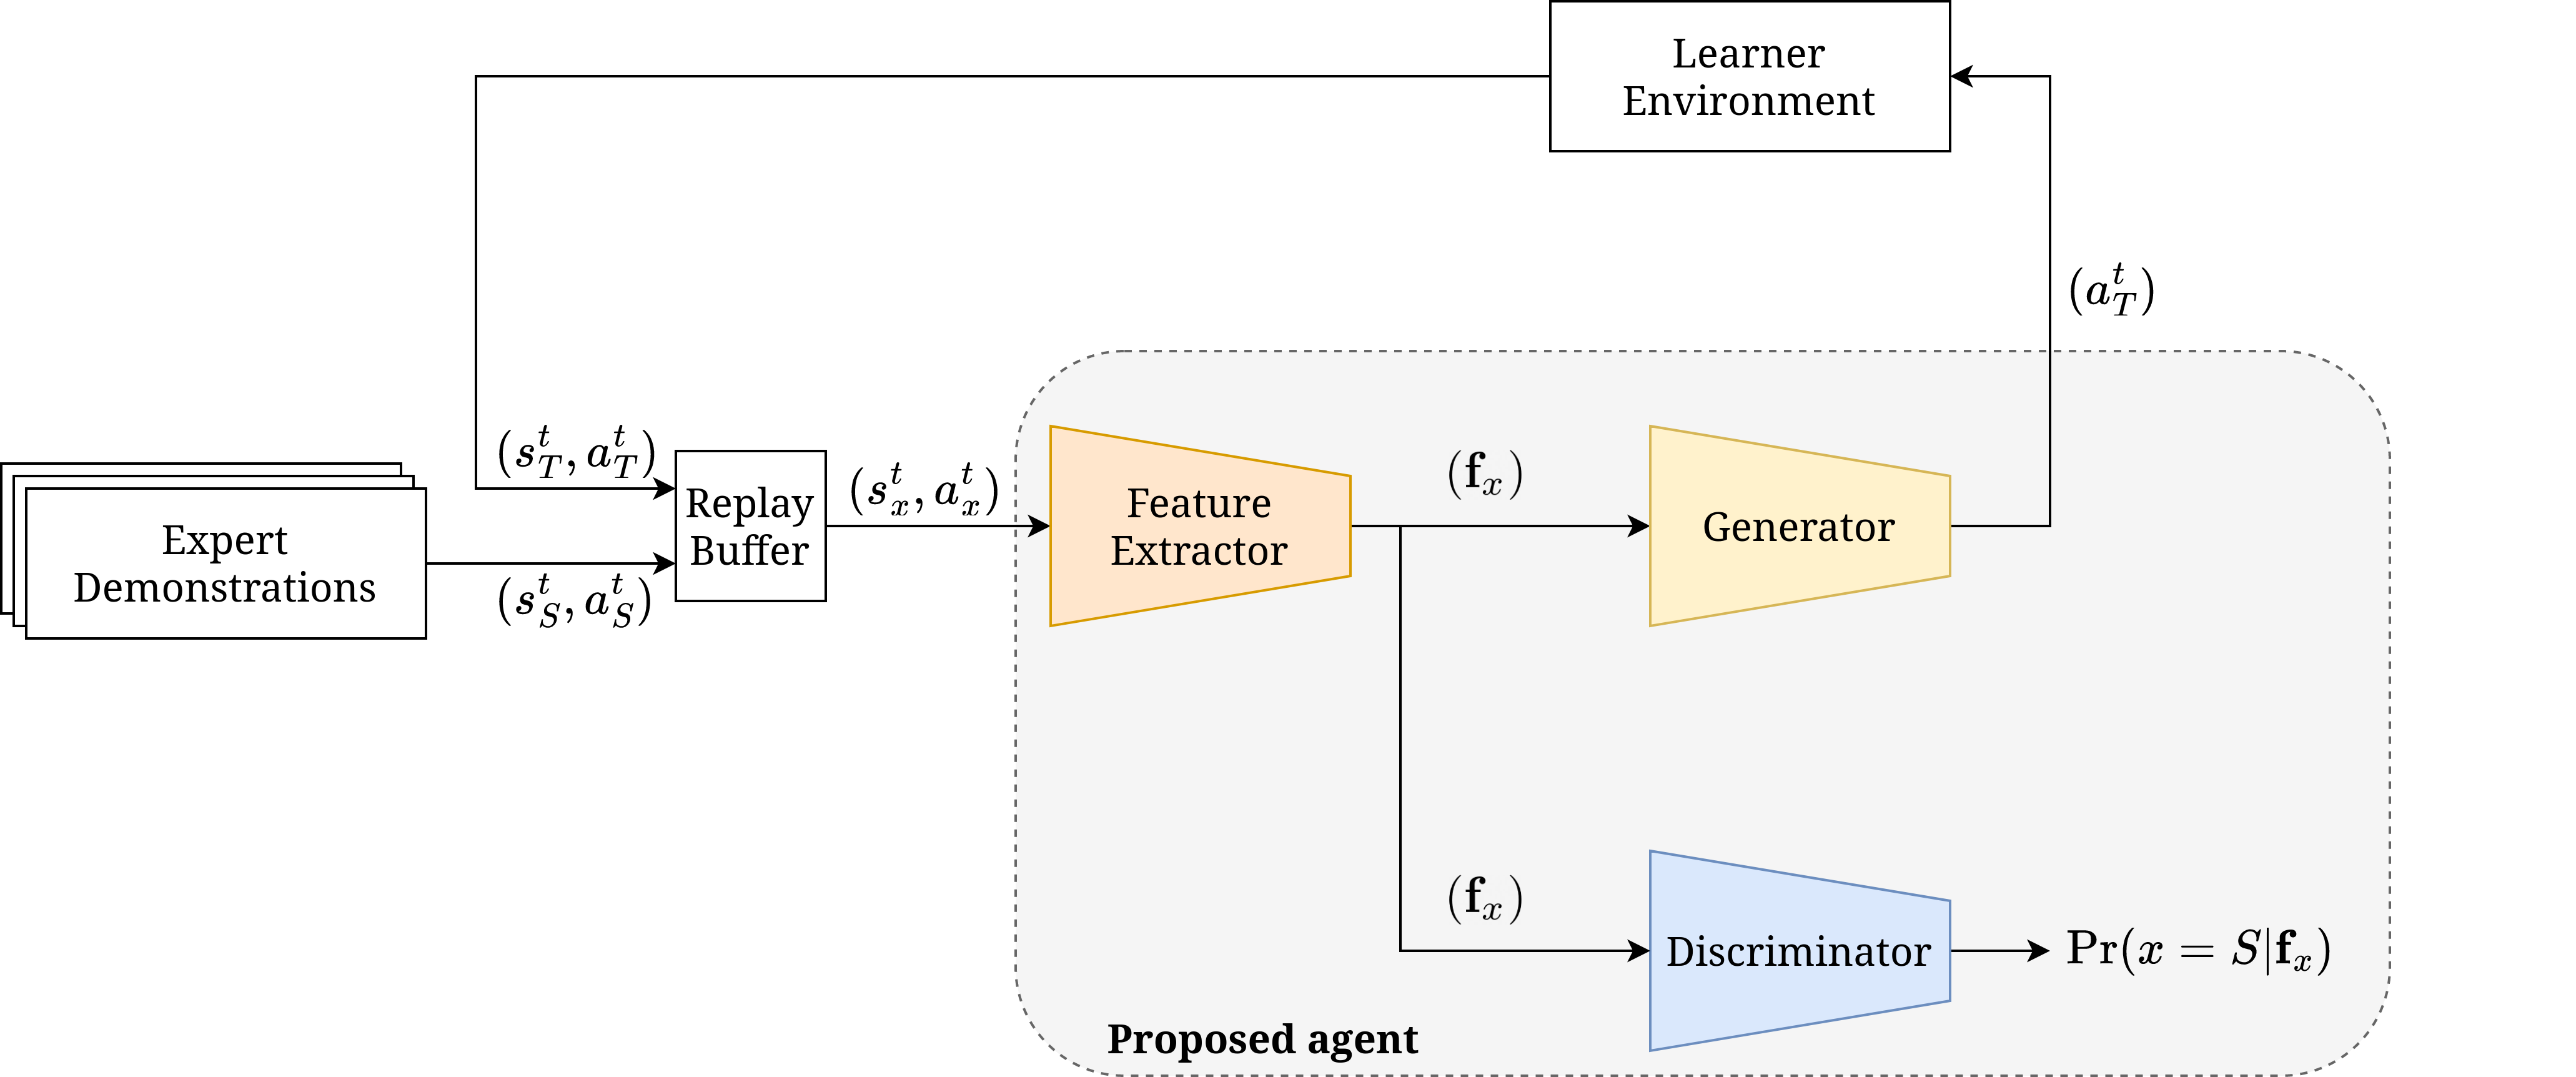
\includegraphics[width=\linewidth]{\FigsDir/new_Architecture.png}
  \caption{\added{The neural network architecture of the proposed \DAIL{} agent.}}
  \label{ch:DAIL:fig:Architecture}
\end{figure}

\subsection{Feature Extractor Network \texorpdfstring{$F$}{F}}
A state-action pair $(s^t_x, a^t_x)$ in domain $x$ is \added{sampled from a replay buffer \cite{zhang2017deeper} and} input to the feature extractor $F$ to produce a feature vector $\mathbf{f}_x=F(s^t_x, a^t_x)$.
$F$ is trained to capture the structural similarities or the shared features between $\mathcal{E}$ and $\mathcal{L}$ domains by minimizing the distance between two features $\mathbf{f}_\mathcal{E}$ and $\mathbf{f}_\mathcal{L}$.
Therefore, the loss function of $F$ is defined as:

\begin{align}
  \mathfrak{L}_F (F, G) & = \mathbb{E} \left[ \left\|
    F(s^t_\mathcal{E}, a^t_\mathcal{E}) - F(s^t_\mathcal{L}, a^t_\mathcal{L})
  \right\| \right]                                    \\
                        & = \mathbb{E} \left[ \left\|
    F(s^t_\mathcal{E}, a^t_\mathcal{E}) - F( s^t_\mathcal{L}, G( F( s^t_\mathcal{E}, a^t_\mathcal{E} ) ) )
    \right\| \right]
  % 1/T \sum^{}_{}{|| f() - f() ||^2_2}
\end{align}


\subsection{Discriminator Network \texorpdfstring{$D$}{D} and Generator Network \texorpdfstring{$G$}{G}}
The discriminator $D$ is designed to distinguish between expert feature vector $\mathbf{f}_\mathcal{E}$ and learner feature vector $\mathbf{f}_\mathcal{L}$.
Specifically,
$D$ receives a feature vector $\mathbf{f}_x$ outputs a probability $\mathrm{Pr}(x=\mathcal{E}|\mathbf{f}_x)$ to classify whether $\mathbf{f}_x$ is from $\mathcal{E}$ or $\mathcal{L}$.
Meanwhile,
the generator $G$ aims to generate an action $a^t_{L}$ so that $\mathbf{f}_\mathcal{L} = F(s^t_\mathcal{L}, a^t_\mathcal{L})$ looks as similar as possible to $\mathbf{f}_\mathcal{E}$.
In the proposed \DAIL{} agent,
the adversarial loss \cite{GAN_Original} is applied for both networks:

\begin{align}
  \mathfrak{L}_{GAN}(G, D) & =
  \mathbb{E}[
    \log{D(F(s^t_\mathcal{E}, a^t_\mathcal{E}))}
  ] + \mathbb{E}[
    \log{(1-D(F(s^t_\mathcal{L}, a^t_\mathcal{L})))}
  ]                                        \\
                           & = \mathbb{E}[
    \log{D(F(s^t_\mathcal{E}, a^t_\mathcal{E}))}
  ] + \mathbb{E}[
    \log{(1-D(F(s^t_\mathcal{L}, G(F(
      s^t_\mathcal{E}, a^t_\mathcal{E}
      )))))}
  ]
\end{align}

The optimal policy is achieved using a RL-based policy gradient,
which relies on reward signal $r=-\log{D(F(s^t_\mathcal{E}, a^t_\mathcal{E}))}$ provided by the learned discriminator.


\subsection{Full Objective}
During the learning phase,
in order to learn domain-shared features between $\mathcal{E}$ and $\mathcal{L}$ domains,
the feature extractor $F$ and the generator $G$ are optimized to minimize the feature extractor loss $\mathfrak{L}_F$.
At the same time,
given a feature vector $\mathbf{f}_x$ of domain $x$,
we want to judge whether $\mathbf{f}_x$ is from $\mathcal{E}$ or $\mathcal{L}$ by minimizing the domain classification loss $\mathfrak{L}_{GAN}$.
This encourages domain-specific features to be captured by $F$.
Overall, the full objective function is:

\begin{align}
   & \underset{F, G}{max} \underset{D}{min} \mathfrak{L}(F, G, D) \\
   & \quad\text{subject to \:}
  \mathfrak{L}(F, G, D) = {\mathfrak{L}_{GAN}(G, D)} - \lambda\mathfrak{L}_F
\end{align}

The goal is to find a saddle point, where:

\begin{align}
  (\hat{F}, \hat{G}) & = \underset{F, G}{argmax}{\mathfrak{L}(F, G, \hat{D})}    \\
  \hat{D}            & = \underset{D}{argmin}{\mathfrak{L}(\hat{F}, \hat{G}, D)} \\
\end{align}

At the saddle point,
the $\hat{D}$ minimizes the domain classification loss.
The feature extractor $\hat{F}$ and the generator $\hat{G}$ minimize the distance between both domains (i.e. the features are shared between domains),
while maximizing the domain classification loss (i.e. the features are specific to each domain).
The parameter $\lambda$ controls the trade-off between domain-shared features and domain-specific features should be learned by $F$.

The learning algorithm of the proposed agent is outlined in Algorithm \ref{ch:DAIL:alg:ProposedModel}.

\begin{algorithm}
  \caption{\DAIL{}}
  \label{ch:DAIL:alg:ProposedModel}

  \begin{algorithmic}[1]
    \Input
    \Desc{$\mathcal{D}_\mathcal{E}$}{A set of expert demonstrations}
    \EndInput

    \State Randomly initialize feature extractor network $F$, generator $G$ and discriminator $D$
    \For {i = 0, 1, 2, ...}
    \State Sample an expert demonstration $\tau^i_\mathcal{E} \sim \mathcal{D}_\mathcal{E}$
    \State Update the parameters of feature extractor network $F$ with the gradient
    \[\mathbf{E}[
        \nabla_F log(D( \mathbf{f}_\mathcal{E} ))
      ] + \mathbf{E}[
        \nabla_F log(1 - D( \mathbf{f}_\mathcal{L} ))
      ] - \lambda \mathbf{E}[
        \nabla_F \left\|
        \mathbf{f}_\mathcal{E} - \mathbf{f}_\mathcal{L}
        \right\|
      ]
    \]
    \State Update the discriminator parameters with the gradient
    \[\mathbf{E}[
        \nabla_D log(D( \mathbf{f}_\mathcal{E} ))
      ] + \mathbf{E}[
        \nabla_D log(1 - D( \mathbf{f}_\mathcal{L} ))
      ]\]
    \State Update policy $\pi_{L}$ with the reward signal $r=-logD(\mathbf{f}_\mathcal{E})$
    \EndFor

    \Output
    \Desc{$\pi_{L}$}{Learned policy for learner domain}
    \EndOutput
  \end{algorithmic}
\end{algorithm}


